%\setlength{\parindent}{0pt}
\documentclass{article}
\usepackage{amsmath}
\usepackage{amssymb}
\usepackage{amsthm}
\usepackage{latexsym}

\usepackage{amsopn}
\DeclareMathOperator{\stab}{Stab}
\DeclareMathOperator{\perm}{Perm}
\DeclareMathOperator{\im}{im}
\DeclareMathOperator{\Aut}{Aut}
\DeclareMathOperator{\Hom}{Hom}
\DeclareMathOperator{\Perm}{Perm}
\DeclareMathOperator{\Frac}{Frac}
\DeclareMathOperator{\Pic}{Pic}
\DeclareMathOperator{\id}{id}
\DeclareMathOperator{\Tr}{Tr}
\DeclareMathOperator{\Spec}{Spec}
\DeclareMathOperator{\Proj}{Proj}
\DeclareMathOperator{\codim}{codim}


\usepackage[dvipsnames]{xcolor}
 
\definecolor{mypink1}{rgb}{0.858, 0.188, 0.478}

%\usepackage{color}
%\definecolor{keywordcolor}{rgb}{0.7, 0.1, 0.1}   % red
%\definecolor{commentcolor}{rgb}{0.4, 0.4, 0.4}   % grey
%\definecolor{symbolcolor}{rgb}{0.0, 0.1, 0.6}    % blue
%\definecolor{sortcolor}{rgb}{0.1, 0.5, 0.1}      % green
%\usepackage{listings}
%\def\lstlanguagefiles{lstlean.tex} 
%\lstset{language=lean}

\usepackage{enumitem}
\usepackage{tikz-cd}

\usepackage{tikz,tkz-euclide}
\usetikzlibrary{arrows,calc,intersections}
\usetkzobj{all}

\usepackage{enumitem}
\usepackage[margin=2.2cm]{geometry}

\newcommand{\ideal}{\ensuremath{\triangleleft}}
\newcommand{\ol}{\ensuremath{\overline}}
\newcommand{\p}{\ensuremath{\mathfrak{p}}}
\newcommand{\m}{\ensuremath{\mathfrak{m}}}
\newcommand{\A}{\ensuremath{\mathbb{A}}}
\newcommand{\Z}{\ensuremath{\mathbb{Z}}}
\newcommand{\C}{\ensuremath{\mathbb{C}}}
\newcommand{\R}{\ensuremath{\mathbb{R}}}
\newcommand{\Q}{\ensuremath{\mathbb{Q}}}
\newcommand{\N}{\ensuremath{\mathbb{N}}}
\newcommand{\F}{\ensuremath{\mathbb{F}}}
\renewcommand{\P}{\ensuremath{\mathbb{P}}}
\newcommand{\Ox}{\mathscr{O}}

\newcommand{\q}{\ensuremath{\mathfrak{q}}}
%\newcommand{\N}{\ensuremath{\mathbb{N}}}

\usepackage{mathrsfs}
%\usepackage{fontspec}
%\usepackage{mathtools}
%\usepackage{unicode-math}

\usepackage{natbib}
\bibliographystyle{humannat}
%\bibliographystyle{unsrtnat}
%\bibliographystyle{abbrvnat}

\theoremstyle{definition}
\newcounter{dummy} \numberwithin{dummy}{section}
\newtheorem{lemma}[dummy]{Lemma}
%\newtheorem*{lemma*}[dummy]{Lemma}
\newtheorem{prop}[dummy]{Proposition}
\newtheorem{defi}[dummy]{Definition}
\newtheorem{cor}[dummy]{Corollary}
\newtheorem{example}[dummy]{Example}
\newtheorem{thm}[dummy]{Theorem}



\newcommand*{\DashedArrow}[1][]{\mathbin{\tikz [baseline=-0.25ex,-latex, dashed,#1] \draw [#1] (0pt,0.5ex) -- (1.3em,0.5ex);}}%
\newcommand{\dto}{\DashedArrow[->,densely dashed]}
%\newcommand{\da}{\DashedArrow}

%\usepackage{microtype}
\usepackage[activate={true,nocompatibility},final,tracking=true,kerning=true,spacing=true,factor=1100,stretch=10,shrink=10]{microtype}
\author{Louis Carlin -- u6384109}
\title{Smooth Schemes of dimension 1}
\usepackage[pdftex]{hyperref}
\hypersetup{
  colorlinks=true
}
\begin{document}
\maketitle

\section{Introduction}
I was first made aware of algebraic geometry in a course on algebraic number theory with Jim Borger in 2018.
In this course we studied the obstructions of factorising ideals in a \textit{number ring} into primes and we developed a method of extending these rings to \textit{rings of integers} where unique prime factorisation of ideals does hold.
For the benefit of students who had already seen a bit of algebraic geometry Jim would draw the rings as one dimension curves where the primes obstructing factorisation were singular points.
He told us that the process of extending a ring to one where factorisation held was geometrically the analogue of \textit{resolving} the singularities on these curves.

\begin{figure}[h]
  \label{resolutionFig}
  \centering
    \tikzset{every picture/.style={line width=0.75pt}} %set default line width to 0.75pt        
    
    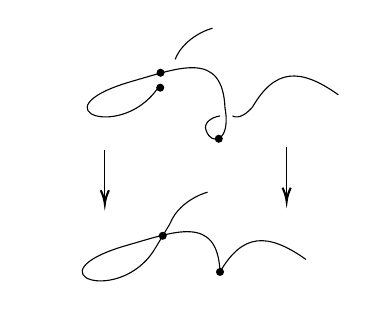
\begin{tikzpicture}[x=0.75pt,y=0.75pt,yscale=-0.6,xscale=0.6]
    %uncomment if require: \path (0,300); %set diagram left start at 0, and has height of 300
    
    %Curve Lines [id:da5284701054564593] 
    \draw    (134.5,245.67) .. controls (173.5,234.67) and (208.5,219.67) .. (210.5,266.67) ;
    %Curve Lines [id:da7183392864588551] 
    \draw    (210.5,266.67) .. controls (228.5,235.67) and (248.5,234.67) .. (279.5,256.67) ;
    %Curve Lines [id:da99364446119495] 
    \draw    (134.5,245.67) .. controls (56.5,268.67) and (130.5,294.67) .. (158.5,247.67) ;
    %Straight Lines [id:da04059644256861805] 
    \draw    (170.5,227.67) -- (158.5,247.67) ;
    %Curve Lines [id:da5835036369344635] 
    \draw    (170.5,227.67) .. controls (175.5,214.67) and (189.5,205.67) .. (200.5,202.67) ;
    %Flowchart: Connector [id:dp676456863598681] 
    \draw  [fill={rgb, 255:red, 0; green, 0; blue, 0 }  ,fill opacity=1 ] (160,106.75) .. controls (160,105.23) and (161.23,104) .. (162.75,104) .. controls (164.27,104) and (165.5,105.23) .. (165.5,106.75) .. controls (165.5,108.27) and (164.27,109.5) .. (162.75,109.5) .. controls (161.23,109.5) and (160,108.27) .. (160,106.75) -- cycle ;
    %Curve Lines [id:da32105592735614374] 
    \draw    (138.5,114) .. controls (177.5,103) and (212.5,88) .. (214.5,135) ;
    %Curve Lines [id:da8814257851885536] 
    \draw    (236.5,134.43) .. controls (254.5,103.43) and (274.5,102.43) .. (305.5,124.43) ;
    %Curve Lines [id:da7431024376674706] 
    \draw    (138.5,114) .. controls (60.5,137) and (134.5,163) .. (162.5,116) ;
    %Curve Lines [id:da23901143687837978] 
    \draw    (174.5,96) .. controls (179.5,83) and (193.5,74) .. (204.5,71) ;
    %Flowchart: Connector [id:dp20942183150561444] 
    \draw  [fill={rgb, 255:red, 0; green, 0; blue, 0 }  ,fill opacity=1 ] (159.75,118.75) .. controls (159.75,117.23) and (160.98,116) .. (162.5,116) .. controls (164.02,116) and (165.25,117.23) .. (165.25,118.75) .. controls (165.25,120.27) and (164.02,121.5) .. (162.5,121.5) .. controls (160.98,121.5) and (159.75,120.27) .. (159.75,118.75) -- cycle ;
    %Curve Lines [id:da4553762848060199] 
    \draw    (214.5,135) .. controls (219.5,162.43) and (203.5,165.43) .. (199.5,153.43) ;
    %Curve Lines [id:da7308092900654524] 
    \draw    (199.5,153.43) .. controls (196.5,147.43) and (203.5,142.43) .. (210.5,141.43) ;
    %Curve Lines [id:da21824928823051848] 
    \draw    (220.5,141.43) .. controls (223,142.86) and (228.5,143.43) .. (236.5,134.43) ;
    %Flowchart: Connector [id:dp19392939956116861] 
    \draw  [fill={rgb, 255:red, 0; green, 0; blue, 0 }  ,fill opacity=1 ] (207.75,266.67) .. controls (207.75,265.15) and (208.98,263.92) .. (210.5,263.92) .. controls (212.02,263.92) and (213.25,265.15) .. (213.25,266.67) .. controls (213.25,268.19) and (212.02,269.42) .. (210.5,269.42) .. controls (208.98,269.42) and (207.75,268.19) .. (207.75,266.67) -- cycle ;
    %Flowchart: Connector [id:dp4860456167453344] 
    \draw  [fill={rgb, 255:red, 0; green, 0; blue, 0 }  ,fill opacity=1 ] (161.75,237.67) .. controls (161.75,236.15) and (162.98,234.92) .. (164.5,234.92) .. controls (166.02,234.92) and (167.25,236.15) .. (167.25,237.67) .. controls (167.25,239.19) and (166.02,240.42) .. (164.5,240.42) .. controls (162.98,240.42) and (161.75,239.19) .. (161.75,237.67) -- cycle ;
    %Flowchart: Connector [id:dp5746113487403737] 
    \draw  [fill={rgb, 255:red, 0; green, 0; blue, 0 }  ,fill opacity=1 ] (206.75,159.75) .. controls (206.75,158.23) and (207.98,157) .. (209.5,157) .. controls (211.02,157) and (212.25,158.23) .. (212.25,159.75) .. controls (212.25,161.27) and (211.02,162.5) .. (209.5,162.5) .. controls (207.98,162.5) and (206.75,161.27) .. (206.75,159.75) -- cycle ;
    %Straight Lines [id:da43158084172872013] 
    \draw    (118,168.43) -- (118,210) ;
    \draw [shift={(118,212)}, rotate = 270] [color={rgb, 255:red, 0; green, 0; blue, 0 }  ][line width=0.75]    (10.93,-3.29) .. controls (6.95,-1.4) and (3.31,-0.3) .. (0,0) .. controls (3.31,0.3) and (6.95,1.4) .. (10.93,3.29)   ;
    %Straight Lines [id:da21013104227019275] 
    \draw    (264,166.43) -- (264,208) ;
    \draw [shift={(264,210)}, rotate = 270] [color={rgb, 255:red, 0; green, 0; blue, 0 }  ][line width=0.75]    (10.93,-3.29) .. controls (6.95,-1.4) and (3.31,-0.3) .. (0,0) .. controls (3.31,0.3) and (6.95,1.4) .. (10.93,3.29)   ;
    
    \end{tikzpicture}
    \caption{A map of one dimensional curves resolving the singularities of the target curve.}
  \end{figure}

At the time I was both fascinated and completely mystified by these pictures.
Why did it make any sense to draw a ring (a completely algebraic object) as a curve (a completely geometric object)?
How were we able to interpret an ideals effect on factorization (an algebraic property) as the smoothness of the corresponding point (a geometric property)?
The goal of this report is to discuss these ideas through the lens of algebraic geometry.
In particular the main objects of interest will be schemes of dimension 1 and their tangent spaces.

Throughtout we will keep two main examples in mind.
The first is the \textbf{nodal cubic} $\Spec \C[x,y](y^2-x^2-x^3)$.
We think of this as the curve $y^2 = x^3 + x^2$ in $\C^2$ which is smooth away from the origin, and we will use this to inspire much of our geometric intuition.
Note that this is a two dimensional over $\R$ and so by calling it a curve we have already abandoned some of our real intuition in favor of the complex picture.

\begin{figure}
  \centering
  
  \tikzset{every picture/.style={line width=0.75pt}} %set default line width to 0.75pt        
  
  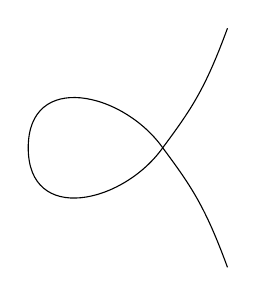
\begin{tikzpicture}[x=0.75pt,y=0.75pt,yscale=-0.6,xscale=0.6]
  %uncomment if require: \path (0,300); %set diagram left start at 0, and has height of 300
  
  %Curve Lines [id:da7005437511354093] 
  \draw    (143.5,119.29) .. controls (143.5,57.29) and (219.5,74.29) .. (251.5,119.29) ;
  %Shape: Boxed Bezier Curve [id:dp5402671719083179] 
  \draw    (143.5,119.29) .. controls (143.5,181.29) and (219.5,164.29) .. (251.5,119.29) ;
  %Curve Lines [id:da6056770531453461] 
  \draw    (251.5,119.29) .. controls (274.5,150.29) and (285.5,166.29) .. (303.5,215.29) ;
  %Shape: Boxed Bezier Curve [id:dp5121004114279468] 
  \draw    (251.5,119.29) .. controls (274.5,88.29) and (285.5,72.29) .. (303.5,23.29) ;
  
  
  
  \end{tikzpicture}
  \caption{The real locus of the nodal cubic. Note the singular point where the curve overlaps.}
  \end{figure}

The second example is $\Spec \Z\left[\frac{1+\sqrt{-3}}{2}\right]$, which we will see this is the ring of integers of $\Q(\sqrt{-3})$..
For convenience we will denote $\frac{1+\sqrt{-3}}{2}$ by $\alpha$.
At first glance this example seems more arithmetic then geometric in nature, but we will see that it too can be thought of as a smooth curve.
Hopefully you will become convinced that these two seemingly quite different rings actually have a lot in common.

% I begin in section \ref{dimSec} with the definition of dimensionality and an explanation of why the rings/schemes we are interested in have dimension 1.
% In section \ref{smoothSec} I introduce the Zariski tangent space in order to give a completely algebraic categorisation of what it means to be smooth.
%Finally in section \ref{ramSec} I discuss ramification, and how we understand it geometrically.




\section{Integrality and the ring of integers}
Since rings of integers are a big motivation for this report we begin with an explanation of what integrality is and what we mean by ring of integers.
The notion of integrality will apply to arbitrary ring extensions, although in algebraic number theory we are typically only interested in a few select types of extension.

%What does it mean to be integral?
Suppose $A \subset B$ is an extension of rings.
We say an element $b \in B$ is \textbf{integral} over $A$ if it is a zero of a monic polynomial
$$x^n + a_{n-1}x^{n-1}+\cdots+a_0$$
with coefficients in $A$.
We say the ring $B$ is \textbf{integral} over $A$ or that the extension is \textbf{integral} if all elements of $B$ are integral over $A$.
The following lemma gives an important characterisation of when elements are integral.
\begin{lemma}
  \label{intFinGenLemma}
  A finite collection of elements $b_1,\ldots,b_k \in B$ are all integral over $A$ if and only if the ring $A[b_1,\ldots,b_k]$ is finitely generated as an $A$-module.
\end{lemma}
\begin{proof}

For the first direction we will consider the case of one element $b \in B$.
The general case follows by induction with not too much work  (see \citeauthor[Prop. 2.2]{neukirch2013algebraic}).
Suppose $b$ is integral over $A$, so there is a monic polynomial $f \in A[x]$ with coefficients in $A$ such that 
$$f(b) = b^n + a_{n-1}b^{n-1} + \cdots + a_0 = 0$$
Since $f$ is monic we can use the division algorithm to write any polynomial $g \in A[x]$ as $fq+r$ where $\deg r < \deg f$.
Thus for any $g(b) \in A[b]$ we have $g(b)= f(b)q(b)+r(b)=r(b)$.
Since $\deg r < \deg f$ we see that $r(b)$ is an $A$-linear combination of $b,\ldots,b^{n-1}$.
This is to say that $b,b^2,\ldots, b^{n-1}$ generate $A[b]$ as an $A$-module.

Conversely, suppose that $A[b_1,\ldots,b_k]$ is finitely generated as an $A$-module with generators $\omega_1, \ldots, \omega_r$.
Then for each $b\in A[b_1,\ldots,b_n]$ and each $i = 1, \ldots, r$ there exist coefficients $a_{ij} \in A$ such that 
$$b \omega_i = \sum_{j=1}^r a_{ij} \omega_j$$
If we let $\omega$ be the vector with components $\omega_j$ then in matrix form this is
$$ \left(bI - (a_{ij})\right)\omega = 0$$
In particular since $\omega$ is nonzero we conclude that
$$ \det \left(bI - (a_{ij})\right) = 0$$
Thus $\det \left(xI - (a_{ij})\right)$ is a monic polynomial with coefficients in $A$ that $b$ is a root of, so $b$ is integral.
\end{proof}
\noindent
As an important consequence we get the following results.
\begin{cor}
  \label{intRingProp}
  Suppose $b_1, b_2 \in B$ are integral over $A$. Then $b_1+b_2$ and $b_1 b_2$ are both integral over $A$.
\end{cor}
\begin{proof}
  The rings $A[b_1,b_2]$ and $A[b_1,b_2,b_1+b_2]$ are isomorphic so if $A[b_1,b_2]$ is finitely generated as an $A$-module then so is $A[b_1,b_2,b_1+b_2]$ and thus $b_1+b_2$ is integral by the previous lemma.
  The same argument works for $A[b_1,b_2]$ and $A[b_1,b_2,b_1b_2]$.
\end{proof}

\begin{cor}
  \label{towerProp}
  Suppose $A \subset B \subset C$ is a tower of ring extensions and that the extension $A \subset B$ is integral.
  Then an element of $C$ is integral over $A$ if and only if it is integral over $B$.
\end{cor}
\begin{proof}
  Suppose $c \in C$ is integral over $A$.
  Then $c$ is the root of a monic polynomial with coefficients in $A$.
  Since $A \subset B$ the coefficients of that polynomial are also in $B$ so $c$ is integral over $B$.

  Conversely suppose that $c \in C$ is integral over $B$ as the root of a polynomial $x^n + b_{n-1}x^{n-1} + \cdots + b_0$.
  Then $c$ is also integral over $A[b_0, \ldots, b_{n-1}]$ as a root of the same polynomial.
  Then by lemma \ref{intFinGenLemma} the ring $A[b_0, \ldots, b_{n-1},c]$ is finitely generated as an $A[b_0, \ldots, b_{n-1}]$-module.
  Since the $b_i$ are integral over $A$ the ring $A[b_0, \ldots, b_{n-1}]$ is a finitely generated $A$ module.
  Putting these two facts together we see that $A[b_0, \ldots, b_{n-1},c]$ is a finitely generated $A$-module and thus use lemma \ref{intFinGenLemma} to conclude that $c$ is integral over $A$.
\end{proof}

Recall that an \textbf{algebraic number field} is a finite extension of $\Q$.
In algebraic number theory we are primarily interested in integral extensions of $\Z$ inside algebraic number fields.
For example, it can be checked that $\alpha=\frac{1+\sqrt{-3}}{2} \in \Q(\sqrt{-3})$ is integral over $\Z$ by showing that it is a root of the monic polynomial $x^2-x+1$.
We see by \ref{intRingProp} that $\Z\left[\alpha\right]$ is integral over $\Z$.

Corollary\ref{intRingProp} tells us that in an extension $A \subset B$ the integral elements form a subring of $B$ that is integral over $A$.
We refer to this ring as the \textbf{integral closure} of $A$ in $B$.
If the integral closure of $A$ in $B$ is just $A$ then we say that $A$ is \textbf{integrally closed} in $B$.
We see by \ref{towerProp} that the integral closure of any integral extension of $A$ in $B$ is the same, and so the integral closure of $A$ is indeed integrally closed.

If $K$ is a number field then the integral closure of $\Z$ in $K$ is known as the \textbf{ring of integers} of $K$ and denoted $\mathcal{O}_K$.
%As claimed earlier $\Z\left[\frac{1+\sqrt{-3}}{2}\right]$ is the ring of integers of $\Q(\sqrt{-3})$.
We will show later on that $\Z\left[\alpha\right]$ is \textit{Dedekind} which implies it is integrally closed in its fraction field thus indeed is its ring of integers.
Conversely we will see that $\C[x,y]/(y^2-x^2-x^3)$ is not \textit{Dedekind} because it has a singular point at $(0,0)$, thus we will conclude that it is not integrally closed in its fraction field.

In general there do exists algorithms for computing rings of integers of arbitrary number fields, although they have poor time complexity linked to the difficulty of factoring large integers.
For ore on this, see \citeauthor{stevenhagen2012number}.


\section{Dimensionality}
\label{dimSec}
To understand why we think of both examples as curves we need to give a suitable definition of dimension.
We might expect that this definition should be algebraic in nature so that it applies to arbitrary schemes.
This is indeed the case, although somewhat surprisingly it can also be thought of as a purely topological condition.
We want this definition to agree with our intuition, with for example $\dim \A^n =n$ and $\dim \P^n=n$.
These things will indeed be true although they won't be demonstrated here.

%definition
We define the \textbf{Krull dimension} or simply \textbf{dimension} of a ring $R$ as the length of the longest chain of strictly ascending prime ideals in $R$, where the count starts at 0.
That is, $\dim R$ is the largest $n$ such that there exists a strictly ascending chain of prime ideals
$$\p_0 \subsetneq \cdots \subsetneq \p_n$$
Recalling that in the affine case prime ideals correspond to irreducible closed subsets, we make the definition that the \textbf{dimension} of a scheme $X$ is the length of the longest chain of irreducible closed subsets of $X$.
Since the correspondence mentioned above is order reversing we find that $\dim R = \dim \Spec R$.
It is worth noting that dimension may be infinite and that this can occur even if $R$ or $X$ are Noetherian.

%codim def
The notion of codimension is more tricky as a scheme can have multiple irreducible components of different dimensions.
One way to circumvent this is to only define codimension of irreducible components.
If $\p$ is a prime in a ring $R$ then the \textbf{height} or \textbf{codimension} of $\p$ is the length $n$ of the longest chain of prime inclusions
$$\p_1 \subsetneq \cdots \subsetneq \p_n \subsetneq \p$$
If $Y \subset X$ is an irreducible closed subset then the \textbf{codimension} of $Y$ is the largest $n$ such that there is a chain of irreducible closed subsets
$$Y \subsetneq Y_1 \subsetneq \cdots \subsetneq Y_n$$
Since these algebraic and geometric definitions of codimension reverse the order of inclusions they also coincide in the affine case.

%why is example 1 dim 1?
\begin{example}
  The ring $\C[x,y]/(y^2-x^2-x^3)$ is one dimensional.
\end{example}
\noindent
We determine the primes of $\C[x,y]/(y^2-x^2-x^3)$.
By the correspondence theorem these correspond to the primes of $\C[x,y]$ containing $y^2-x^2-x^3$.
The primes of $\C[x,y]$ are either generated by a single irreducible polynomial or are of the form $(x-a,y-b)$ for $a,b \in \C$.
Since $y^2-x^2-x^3$ is irreducible the only prime of the first form containing $y^2-x^2-x^3$ is $(y^2-x^2-x^3)$ which corresponds to $(0)$ in $\C[x,y]/(y^2-x^2-x^3)$.
The primes of the second form containing $y^2-x^2-x^3$ are exactly the closed points $(a,b)$ lying on the curve $y^2=x^2+x^3$.
Thus the longest chain of prime inclusions is
$$ (0) \subset (a,b)$$
and so $\C[x,y]/(y^2-x^2-x^3)$ is indeed one dimensional.
$\hfill\blacksquare$

%Why do rings of integers have dim 1?
\begin{example}
  The ring $\Z\left[\alpha\right]$ is one dimensional.
\end{example}
\noindent
We determine the primes of $\Z\left[\alpha\right] \cong \Z[x]/(x^2-x+1)$.
By the correspondence theorem these are the primes of $\Z[x]$ containing $x^2-x+1$, so now we need to understand the primes of $\Z[x]$.
We break this analysis into cases.
\begin{itemize}
  \item \textbf{Case 1: $\p$ is a prime of $\Z[x]$ containing a nonzero integer}:
  
  If $\p$ contains any nonzero integer then by primality $\p$ must contain at least one prime integer $p \in \Z$.
  In fact it cannot contain two different primes as then Euclid's algorithm would show that it also contained 1.
  If $\p$ contains the prime $p$ then it corresponds to a prime in $\F_p[x]$.
  The primes in $\F_p[x]$ are the generic prime $(0)$ and the primes generated by a single polynomial irreducible in $\F_p$.
  Lifting this back up we see that either $\p = (p)$ or $\p = (p,f(x))$ where $f(x)$ is any lift of an irreducible polynomial in $\F_p[x]$.

  \item \textbf{Case 2: $\p$ is a prime of $\Z[x]$ not containing a nonzero integer:}
  
  We will show that $\p$ is either zero or generated by a single irreducible polynomial in $\Z[x]$.
  Suppose not so that there exist $f,g \in \p$ with no common factors.
  Then in particular $f$ and $g$ are coprime over $\Q$ and so there exist $\frac{a_1}{b_1},\frac{a_2}{b_2} \in \Q$ such that $\frac{a_1}{b_1}f + \frac{a_2}{b_2}g=1$.
  Clearing denominators we see that $a_1b_2f + a_2b_1g = b_1b_2$, which is a contradiction as it implies that the integer $b_1b_2$ is in $\p$.
\end{itemize}
From the above analysis we see that the primes in $\Z[x]$ containing $x^2-x+1$ are $(x^2-x+1)$ and $(p, g(x))$ where $g(x)$ is a factor of $x^2-x+1$ mod $p$.
The prime $(x^2-x+1)$ corresponds to $(0)$ in $\Z\left[\alpha\right]$ and the other primes correspond to $\left(p, g\left(\alpha\right)\right)$.
Note that when $x^2-x+1$ is irreducible mod $p$ we have $(p, g(\alpha))=(p,0)=(p)$.
In general, for a fixed $p$, primes of the form $(p, g(\alpha))$ be related to each other by strict inclusions as no such inclusions exist in $\F_p[x]$.
Then can be no other containments since as explained above prime ideals contain only one prime integer.
Thus the longest chain of primes is
$$ (0) \subset \left(p, g\left(\alpha\right)\right)$$
and so we conclude that $\dim \Z\left[\alpha\right] = 1$.

The analysis here generalises immediately to show that rings of the form $\Z[\alpha]$ for integral $\alpha$ are dimension one.
It is also a good illustration of the fact that understanding the behaviour of primes in these rings is the same as understanding the factorisation of polynomials mod $p$. 
It is less simple to see that arbitrary rings of integers are dimension one, although this is indeed the case.
$\hfill\blacksquare$

\section{Regularity}
\label{smoothSec}
In our drawings we have been picturing both examples as smooth curves. In the function field example this makes intuitive sense as away from the origin it is smooth as a complex manifold.
We need a sensible definition of smoothness which will formalise this intuition and motivate our understanding of the arithmetic example as a smooth object.
To this end we construct a \textit{Zariski tangent space} inspired by the tangent space of differential geometry but defined purely algebraically.
We will end up giving a definition of regularity rather than smoothness, which is a similar but not identical concept.
%TODO are they the same in dim 1?

In differential geometry one definition of the tangent space of a smooth manifold is in terms of \textit{derivations}.
We think of a derivation at a point $p$ as an operator which allows us to evaluate the derivative of differentiable functions at $p$ in a particular direction.
More concretely, suppose $M$ is a smooth manifold with sheaf of differentiable functions $\Ox$. 
Then the \textbf{derivations} at a point $p \in M$ are the $\R$-vector space homomorphisms $D:\Ox_p \to \R$ satisfying the Leibnitz rule
$$D(fg) = fDg + gDf$$
The elements of $\Ox_p$ are differentiable functions on some neighbourhood of $p$ and thus we think of them as the value they take at $p$ plus some information about the derivatives of $p$.
It is not too hard to see that derivations depend only on the differential information and thus agree with our intuition of them as directional derivative operators.
The \textbf{tangent space} of $M$ at a point $p$ is the $\R$-vector space of derivations at $p$ and is denoted $T_pM$.
In the case where $M$ is embedded in $\R^n$ this definition agrees with our geometric intuition of the tangent plane to $M$.

%alternate definition of tangent space
Inspired by the algebraic nature of this definition we make a similar definition for a scheme $X$.
If $\p$ is a point in $X$ then a \textbf{derivation} at $\p$ is a $\kappa(\p)$-vectorspace map $\Ox_{X,\p} \to \kappa(\p)$ satisfying the Leibnitz rule.
The \textbf{Zariski tangent space} of $X$ at $\p$, denoted $T_\p X$, is the $\kappa(\p)$ vector space of derivations at $\p$. Since it is not immediately obvious how to determine what the derivations at a point are we would like an alternate description which is more constructive.
\begin{prop}
  Suppose $\p$ is a point in a scheme $X$ and $\m$ is the maximal ideal of the local ring $\Ox_{X,\p}$. Then there is an isomorphism of $\kappa(\p)$ vectorspaces $T_\p X \cong (\m/\m^2)^\vee$ given by restriction.
\end{prop}
\begin{proof}
  Suppose $D: \Ox_{X,\p} \to \kappa(\p)$ is a derivation.
  Then by restriction we get a map $D': \m \to \kappa(\p)$.
  If $f \in \m^2$ then we can write $f = \sum_i g_ih_i$ for $g_i, h_i \in \m$ and so
  $$ D f = D\left(\sum_i g_ih_i\right)= \sum_i D (g_i h_i) = \sum_i \left( g_i D h_i + h_i Dg_i \right)$$
  In the summand on the right each term is a multiple of something in $\m$ and thus is zero in $\kappa(\p) \cong \Ox_{X,\p}/\m$ and so $D'$ takes elements of $\m^2$ to zero, which is to say it is a map in $(\m/\m^2)^\vee$.
  We note here that restriction is indeed $\kappa(\p)$ linear in the input map $D$.

  Conversely, suppose $D': \m/\m^2 \to \kappa(\p)$.
  We extend $D'$ to a map $D:\Ox_{X,\p} \to \kappa(\p)$ by composing with the map $\Ox_{X,\p} \to \m$ which sends $f$ to $f-f(\p)$.
  To show that $D$ is a derivation let $f,g \in \Ox_{X,\p}$ and note that $(f-f(\p))(g-g(\p)) \in \m^2$.
  Then
  \begin{align*}
    0
    &= D'(f-f(\p))(g-g(\p))\\
    &= D'(fg -f(\p)g -g(\p)f + f(\p)g(\p))\\
    &= D'(fg - f(\p)g(\p)) -f(\p)D'(g-g(\p)) -g(\p)D'(f-f(\p))\\
    &= D(fg) -f(\p)D(g) - g(\p)D(f)
  \end{align*}
  Since $f(\p)$ is how we view $f$ as an element of $\kappa(\p)$ and similarly for $g(\p)$ this is exactly the Leibnitz rule and so $D$ is indeed a derivation.

  We need to show that composing these two maps in either order gives the identity.
  Since the map $\Ox_{X,\p} \to \m$ is an isomorphism on $\m$, if we first extend $D'$ to $D$ then restrict we get $D'$ again.
  Conversely, if we start by restricting $D$ to $D'$ and then extend this to $D''$ we have 
  $$D''(f)=D'(f-f(\p))=D(f-f(\p))=D(f)-D(f(\p))$$
  so it suffices to show that $D(f(\p))$ is zero.
  To do this we note that the Leibnitz rule gives $D(1) = 1 D(1) + 1D(1)$ and so we must have $D(1)=0$.
  Then by $\kappa(\p)$ linearity we have $D(f(\p))= f(\p)D(1)=0$.
\end{proof}

%definition of regular
With this more explicit description of the Zariski tangent space we return to the problem of defining an algebraic notion of regularity.
In differential geometry one way of defining regularity at a point is by the dimension of the tangent space at that point.
If $p$ is a point in an $n$-dimensional smooth manifold $M$ we have $\dim T_p M = n$, which intuitively makes sense as there are $n$ different directions to differentiate along in a neighbourhood of $p$.
If we allow the possibility that $M$ has singular points then we only get an inequality $\dim T_p M \geq n$ and the \textbf{regular points} are exactly the ones where equality holds.

The above definition of a regular point is purely algebraic and so we attempt to adapt it to schemes.
We need to be careful for a few reasons.
With schemes the notion of dimension we gave was a global notion, but intuitively regularity at a point should depend only on local dimension around that point.
Furthermore, the nonclosed points of a scheme are thought of as having higher dimension and thus we would expect the number of tangent directions to these points to be lower and want this to be represented in our definition.
The answer to both these issues is to use the codimension of the point.
If $\p$ is a point in a Noetherian scheme $X$ then we find that 
$$\dim T_\p X \geq \codim \p$$
(see \citeauthor[12.2.1]{vakil2017rising}).
When equality holds we say $\p$ is a \textbf{regular point} and otherwise it is \textbf{singular}.
A scheme is \textbf{regular} if it is regular at every point.

Recall that if $\p$ is a prime in $A$ then $\codim \p$ is the length of the longest chain of prime ideals in $A$ that are contained in $\p$.
Primes in $A_\p$ correspond to primes in $A$ contained in $\p$ and this correspondence is inclusion preserving.
Thus chains of primes contained in $\p$ correspond to chains of primes in $A_\p$.
We also know that $\dim(\m/\m^2)^\vee = \dim (\m/\m^2)$.
Thus we may equivalently check regularity by seeing whether equality holds in
$$\dim (\m/\m^2) \geq \dim \Ox_{X,\p}$$
To simplify\footnote{Or complicate if this is your first time seeing all this!} terminology even further we say a local ring $R$ with maximal ideal $\m$ is \textbf{regular} if $\dim(\m/\m^2) = \dim R$.
Thus a point $\p$ of a scheme is regular if the stalk at that point is regular.

One of the very nice things about dimension one is that there are many different equivalent definitions of regularity.
We will state one here without proof as it relies on some machinery.
A proof can be found in (\citeauthor[12.5]{vakil2017rising}) along with five other equivalent definitions of regularity for one dimensional rings.

\begin{prop}
  A Noetherian local ring of dimension one is regular if and only if its maxmial ideal $\m$ is principal.
\end{prop}

\begin{example}
  $\Spec \C[x,y]/(y^2-x^2-x^3)$ is regular away from $(0,0)$.
  \label{geoSmoothEx}
\end{example}
\noindent
Since $y^2-x^2-x^3$ is irreducible $\C[x,y]/(y^2-x^2-x^3)$ is an integral domain.
Thus $(0)$ is regular since the stalk at $(0)$ is the fraction field of $\C[x,y]/(y^2-x^2-x^3)$, with dimension $0 = \dim (0)/(0)^2$.

The other primes are of the form $(x-a, y-b)$ with $a,b$ on the curve $y^2 - x^2 -x^3$.
The maximal ideal in the corresponding stalk is also generated by $x-a$ and $y-b$ and so to show it is actually principally generated we will show one of the generators is a multiple of the other.
We will first show this for the case $a \neq 0$ except the point $(-1,0)$, and then we will cover this point separately.
The reason the proof works like this is we are essentially using regularity of the intersection with the line $x=a$, which fails at $(-1,0)$.
Amazingly we will see the same idea work for the arithmetic example.
\begin{figure}[h]
  \centering




  \tikzset{every picture/.style={line width=0.75pt}} %set default line width to 0.75pt        

  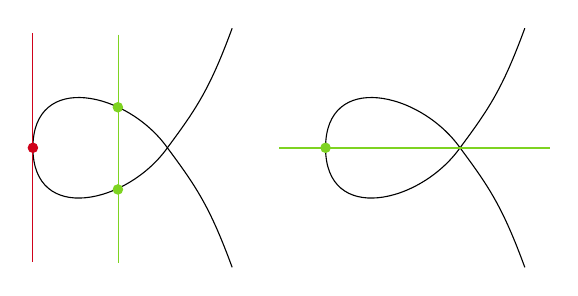
\begin{tikzpicture}[x=0.75pt,y=0.75pt,yscale=-0.6,xscale=0.6]
  %uncomment if require: \path (0,300); %set diagram left start at 0, and has height of 300
  
  %Curve Lines [id:da7005437511354093] 
  \draw    (143.5,119.29) .. controls (143.5,57.29) and (219.5,74.29) .. (251.5,119.29) ;
  %Shape: Boxed Bezier Curve [id:dp5402671719083179] 
  \draw    (143.5,119.29) .. controls (143.5,181.29) and (219.5,164.29) .. (251.5,119.29) ;
  %Curve Lines [id:da6056770531453461] 
  \draw    (251.5,119.29) .. controls (274.5,150.29) and (285.5,166.29) .. (303.5,215.29) ;
  %Shape: Boxed Bezier Curve [id:dp5121004114279468] 
  \draw    (251.5,119.29) .. controls (274.5,88.29) and (285.5,72.29) .. (303.5,23.29) ;
  %Straight Lines [id:da5231216189232124] 
  \draw [color={rgb, 255:red, 208; green, 2; blue, 27 }  ,draw opacity=1 ]   (143.5,27.43) -- (143.5,211.14) ;
  %Straight Lines [id:da5519975969228899] 
  \draw [color={rgb, 255:red, 126; green, 211; blue, 33 }  ,draw opacity=1 ]   (212.5,28.43) -- (212.5,212.14) ;
  %Curve Lines [id:da2716651534997605] 
  \draw    (378.5,119.29) .. controls (378.5,57.29) and (454.5,74.29) .. (486.5,119.29) ;
  %Shape: Boxed Bezier Curve [id:dp8993274445695958] 
  \draw    (378.5,119.29) .. controls (378.5,181.29) and (454.5,164.29) .. (486.5,119.29) ;
  %Curve Lines [id:da9091958158839282] 
  \draw    (486.5,119.29) .. controls (509.5,150.29) and (520.5,166.29) .. (538.5,215.29) ;
  %Shape: Boxed Bezier Curve [id:dp5411608835909054] 
  \draw    (486.5,119.29) .. controls (509.5,88.29) and (520.5,72.29) .. (538.5,23.29) ;
  %Straight Lines [id:da8278974990650314] 
  \draw [color={rgb, 255:red, 126; green, 211; blue, 33 }  ,draw opacity=1 ]   (341.5,119.43) -- (558.5,119.43) ;
  %Shape: Circle [id:dp926025186967611] 
  \draw  [color={rgb, 255:red, 126; green, 211; blue, 33 }  ,draw opacity=1 ][fill={rgb, 255:red, 126; green, 211; blue, 33 }  ,fill opacity=1 ] (208,86.75) .. controls (208,84.68) and (209.68,83) .. (211.75,83) .. controls (213.82,83) and (215.5,84.68) .. (215.5,86.75) .. controls (215.5,88.82) and (213.82,90.5) .. (211.75,90.5) .. controls (209.68,90.5) and (208,88.82) .. (208,86.75) -- cycle ;
  %Shape: Circle [id:dp2273574431432257] 
  \draw  [color={rgb, 255:red, 208; green, 2; blue, 27 }  ,draw opacity=1 ][fill={rgb, 255:red, 208; green, 2; blue, 27 }  ,fill opacity=1 ] (139.75,119.29) .. controls (139.75,117.21) and (141.43,115.54) .. (143.5,115.54) .. controls (145.57,115.54) and (147.25,117.21) .. (147.25,119.29) .. controls (147.25,121.36) and (145.57,123.04) .. (143.5,123.04) .. controls (141.43,123.04) and (139.75,121.36) .. (139.75,119.29) -- cycle ;
  %Shape: Circle [id:dp7765713378703565] 
  \draw  [color={rgb, 255:red, 126; green, 211; blue, 33 }  ,draw opacity=1 ][fill={rgb, 255:red, 126; green, 211; blue, 33 }  ,fill opacity=1 ] (208,152.75) .. controls (208,150.68) and (209.68,149) .. (211.75,149) .. controls (213.82,149) and (215.5,150.68) .. (215.5,152.75) .. controls (215.5,154.82) and (213.82,156.5) .. (211.75,156.5) .. controls (209.68,156.5) and (208,154.82) .. (208,152.75) -- cycle ;
  %Shape: Circle [id:dp7408712442623921] 
  \draw  [color={rgb, 255:red, 126; green, 211; blue, 33 }  ,draw opacity=1 ][fill={rgb, 255:red, 126; green, 211; blue, 33 }  ,fill opacity=1 ] (374.75,119.29) .. controls (374.75,117.21) and (376.43,115.54) .. (378.5,115.54) .. controls (380.57,115.54) and (382.25,117.21) .. (382.25,119.29) .. controls (382.25,121.36) and (380.57,123.04) .. (378.5,123.04) .. controls (376.43,123.04) and (374.75,121.36) .. (374.75,119.29) -- cycle ;
  
  
  
  
  \end{tikzpicture}
  \caption{A geometric interpretation of the proof of example 4.3.}
\end{figure}

Let $f(x,y) = y^2-x^2-x^3$ and suppose $f(a,b)=0$.
When $a$ is not zero or negative one we have $a^2+a^3 \neq 0$ and so $b$ must also be nonzero.
In particular $b$ and $-b$ are distinct roots of $f(a,y)$.
In other words $f(x,y)$ factors into $(y-b)(y+b)$ mod $x-a$ and so we have $f(x,y)=(y-b)(y+b)+(x-a)s(x,y)$ for some $s(x,y)$.
In $\C[x,y]/(f(x,y))$ this is the equation
$$0 = (y-b)(y+b)+(x-a)s(x,y)$$
The prime $(x-a,y-b)$ does not contain $y+b$ since if so it would contain $y-b-(y+b)=2b$ and thus be the unit ideal.
From this we conclude that $y+b$ is invertible in the stalk there and then by rearranging we get $y-b = (x-a)s(x,y)(y+b)^{-1}$, which is to say that $y-b$ is a redundant generator.

The proof is similar at $(-1,0)$ except we are intersecting with the line $y=0$.
Mod $y^2-x^2-x^3$ we have 
$$y^2 = x^2(x+1)$$
The prime $(x+1,y)$ does not contain $x^2$ as otherwise it would contain $1=(x+1)(1-x)+x^2$, thus in the stalk at that prime we have $x+1 = y^2x^{-2}$ and so the generator $x+1$ is redundant.

As we would expect the same idea fails at $(0,0)$ since we find that $x(x+1)$ is in $(x,y)$ and thus not invertible in the stalk there.
Since $\C[x,y]/(y^2-x^2-x^3)$ is an integral domain we may pass to the fraction field to see this is the only possible algebraic relationship between the generators $x$ and $y$ and thus both generators are necessary.
This is to say that $(0,0)$ is not a regular point.
$\hfill\blacksquare$

The proof given in the previous example is somewhat convoluted and a more standard approach would be to appeal to a condition on the corank of the Jacobian.
This proof only works for closed points so again it is a quirk of dimension one.
More generally there is a notion of \textbf{smoothness} for $k$-schemes which is based on this Jacobian condition for points of any dimension and agrees with regularity in dimension one.
I avoided this approach because it requires even more background machinery and because it doesn't really illuminate the connection with the arithmetic example.

\begin{example}
  $\Spec \Z\left[\frac{1+\sqrt{-3}}{2}\right]$ is regular.
\end{example}
\noindent
We first note that $(0)$ is dimension zero in $\Z[\alpha]_{(0)} \cong \Q(\sqrt{-3})$ and thus indeed regular.

Now recall that the nonzero primes of $\Z[\alpha]$ are of the form $\p = (p, g(\alpha))$ where $\overline{g(x)}$ divides $x^2-x+1$ mod p.
The maximal ideal of the stalk at this prime $\Z[\alpha]_\p$ is also generated by $p$ and $g(\alpha)$ and usually denoted $\p\Z[\alpha]_\p$.
I claim that if $\overline{g(x)}$ divides $x^2-x+1$ with multiplicity one then $\p\Z[\alpha]_\p$ is generated by $p$, which would imply that $\Z[\alpha]_\p$ is regular.
To see this we use the fact that $g(x)$ divides $x^2-x+1$  mod $p$ to write
$$x^2-x+1=q(x)g(x)+ps(x)$$
in $\Q[x]$.
Then if $\overline{g(x)}$ only divides $x^2-x+1$ once it does not divide $\overline{q(x)}$ and so $q_i(\alpha)$ is not in $\p$.
Thus $q_i(\alpha)$ is invertible in $\Z[\alpha]_\p$.
If we evalute the above equality with $x=\alpha$ we get
$0 = q(\alpha)g(\alpha) + p s(\alpha)$.
Rearranging gives $g(\alpha) = p s(\alpha) q(\alpha)^{-1}$ which shows that $g(\alpha)$ is a redundant generator and $p$ alone suffices.
Note that essentially we have given the same proof as in example 4.3; geometrically we are taking regularity from the regularity of the intersection with $V(p)$.

We need to determine which primes $\p$ do not satisfy the hypothesis of the previous proof.
That is, for which $p$ does $x^2-x+1$ have a multiple factor mod $p$?
If a polynomial has a multiple factor then the product rule implies this is also a factor of its symbolic derivative.
Using Euclid's algorithm we compute that
$$x^2-x+1 + \left(\frac14 - \frac12 x\right)(2x-1) = \frac{3}{4}$$
and so clearing denominators we have 
$$4(x^2-x+1)+ (1 -2x)(2x-1) = 3$$
Thus $x^2-x+1$ and its derivative $2x-1$ have a common factor mod $p$ only when this root divides $3$ mod $p$.
For nontrivial factors this occurs only when $p=3$, which is to say that primes ``above'' primes $p\neq 3$ are regular. 

Mod 3 we factor $x^2-x+1=(x-2)^2$ and so there is a single prime $\p_3 = (3, \alpha-2)$ above $3$.
In this case we see that
\begin{align*}
  (\alpha-2)(-1-\alpha)
  &= \frac{-3+\sqrt{-3}}{2} \frac{-3-\sqrt{-3}}{2}\\
  &= \frac{9 + 3}{4}\\
  &= 3
\end{align*}
and so $\p_3$ is principal, which implies that $\p_3 \Z[\alpha]_{\p_3}$ is also principal.
Thus $\Z[\alpha]$ is indeed regular at each prime and so $\Spec \Z[\alpha]$ is a regular curve.
$\hfill\blacksquare$

The previous proof can be adapted to understand which primes are regular in any ring $\Z[x]/(f(x))$ for $f(x)$ irreducible, resulting what is known as the Kummer-Dedekind criterion.
\citeauthor{stevenhagen2012number} gives a more detailed explanation of this in chapter 3 and is in general a great computationally minded introduction to the arithmetic theory.

\section{Resolution of singularities}
\label{dedekind}
A \textbf{Dedekind domain} is a one-dimensional Noetherian integral domain $R$ such that for every prime $\p$ of $R$ the localisation $R_\p$ is regular. 
Thus Dedekind domains are the algebraic analogue of regular integral one-dimensional schemes.
More specifically, any affine open subscheme of a regular integral one-dimensional scheme is Dedekind.
Another reason we care about Dedekind domains, especially in number theory, is that they are exactly the rings where we have unique factorization into prime ideals.

The next theorem relates Dedekind domains to the previous discussion of integral closures.
\begin{thm}
  \label{dedeThm}
  A ring $R$ is a Dedekind domain if and only if all of the following hold:
  \begin{itemize}
    \item $R$ is Noetherian;
    \item $R$ has dimension at most one;
    \item $R$ is an integral domain;
    \item $R$ is integrally closed inside its fraction field.
  \end{itemize}
\end{thm}

These conditions are sometimes  taken as the definition of a Dedekind domain.
Most of the work required in proving Theorem \ref{dedeThm} is establishing the following equivalent definition of regularity (see \citeauthor[12.5.8g]{vakil2017rising}).
\begin{prop}
  A Noetherian local ring of dimension one is regular if and only if it is an integral domain that is integrally closed in its fraction field.
\end{prop}

The integral closure of $R$ inside its fraction field is called its \textbf{normalization} and denoted $\widetilde{R}$.
The upshot of Theorem \ref{dedeThm} is that taking the normalization of a one dimensional Noetherian integral domain $R$ gives us its smallest regular extension. 
Geometrically we picture $\Spec \widetilde{R}$ as a smooth curve projecting down to $R$ as in figure \ref{resolutionFig}.
Above already regular primes the primes are essentially the same and so the map does not change these parts of the curve.
Thus we think of taking the normalization as resolving the singularities of $R$.

\begin{example}
  The integral closure of $\C[x,y]/(y^2-x^2-x^3)$ inside its fraction field can be thought of as $\C[t]$ via the map $\C[x,y]/(y^2-x^2-x^3) \to \C[t]$ defined by
  \begin{align*}
    x &\mapsto t^2-1\\
    y &\mapsto t(t^2-1)
  \end{align*}
  This resolves the singularity at $(0,0)$ as in figure 4.
  $\hfill\blacksquare$
\end{example}

\begin{figure}[h]
\label{nodalResFig} 
\centering
\tikzset{every picture/.style={line width=0.75pt}} %set default line width to 0.75pt        

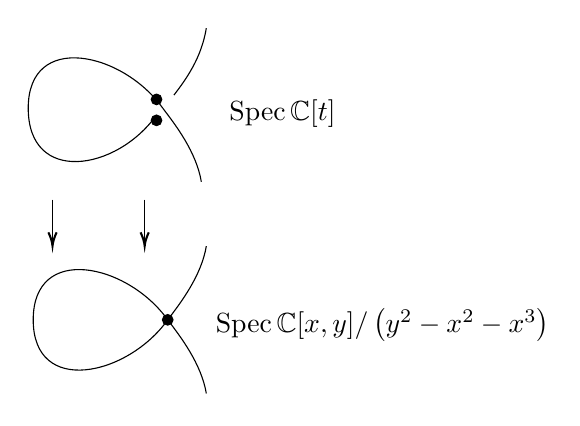
\begin{tikzpicture}[x=0.75pt,y=0.75pt,yscale=-0.6,xscale=0.6]
%uncomment if require: \path (0,359); %set diagram left start at 0, and has height of 359

%Curve Lines [id:da7005437511354093] 
\draw    (143.5,252.29) .. controls (143.5,190.29) and (219.5,207.29) .. (251.5,252.29) ;
%Shape: Boxed Bezier Curve [id:dp5402671719083179] 
\draw    (143.5,252.29) .. controls (143.5,314.29) and (219.5,297.29) .. (251.5,252.29) ;
%Shape: Boxed Bezier Curve [id:dp3203678330728805] 
\draw    (251.5,252.29) .. controls (261.5,265.43) and (278.5,287.43) .. (282.5,311.43) ;
%Shape: Boxed Bezier Curve [id:dp46816703526862513] 
\draw    (251.5,252.29) .. controls (261.5,239.14) and (278.5,217.14) .. (282.5,193.14) ;
%Curve Lines [id:da624388277189942] 
\draw    (139.5,82.29) .. controls (139.5,20.29) and (215.5,37.29) .. (247.5,82.29) ;
%Curve Lines [id:da05077455246129303] 
\draw    (139.5,82.29) .. controls (139.5,144.29) and (210.5,132.86) .. (242.5,87.86) ;
%Shape: Boxed Bezier Curve [id:dp7748218086953953] 
\draw    (247.5,82.29) .. controls (257.5,95.43) and (274.5,117.43) .. (278.5,141.43) ;
%Curve Lines [id:da6056770531453461] 
\draw    (256.5,71.86) .. controls (266.5,58.71) and (278.5,42.14) .. (282.5,18.14) ;
%Shape: Circle [id:dp516031470391844] 
\draw  [fill={rgb, 255:red, 0; green, 0; blue, 0 }  ,fill opacity=1 ] (247.25,252.29) .. controls (247.25,249.94) and (249.15,248.04) .. (251.5,248.04) .. controls (253.85,248.04) and (255.75,249.94) .. (255.75,252.29) .. controls (255.75,254.63) and (253.85,256.54) .. (251.5,256.54) .. controls (249.15,256.54) and (247.25,254.63) .. (247.25,252.29) -- cycle ;
%Shape: Circle [id:dp35351599494319697] 
\draw  [fill={rgb, 255:red, 0; green, 0; blue, 0 }  ,fill opacity=1 ] (238.25,75.29) .. controls (238.25,72.94) and (240.15,71.04) .. (242.5,71.04) .. controls (244.85,71.04) and (246.75,72.94) .. (246.75,75.29) .. controls (246.75,77.63) and (244.85,79.54) .. (242.5,79.54) .. controls (240.15,79.54) and (238.25,77.63) .. (238.25,75.29) -- cycle ;
%Shape: Circle [id:dp5360050124483207] 
\draw  [fill={rgb, 255:red, 0; green, 0; blue, 0 }  ,fill opacity=1 ] (238.25,92.11) .. controls (238.25,89.76) and (240.15,87.86) .. (242.5,87.86) .. controls (244.85,87.86) and (246.75,89.76) .. (246.75,92.11) .. controls (246.75,94.45) and (244.85,96.36) .. (242.5,96.36) .. controls (240.15,96.36) and (238.25,94.45) .. (238.25,92.11) -- cycle ;
%Straight Lines [id:da030297809466028225] 
\draw    (159,155.86) -- (159,191) ;
\draw [shift={(159,193)}, rotate = 270] [color={rgb, 255:red, 0; green, 0; blue, 0 }  ][line width=0.75]    (10.93,-3.29) .. controls (6.95,-1.4) and (3.31,-0.3) .. (0,0) .. controls (3.31,0.3) and (6.95,1.4) .. (10.93,3.29)   ;
%Straight Lines [id:da12488812741406363] 
\draw    (233,155.86) -- (233,191) ;
\draw [shift={(233,193)}, rotate = 270] [color={rgb, 255:red, 0; green, 0; blue, 0 }  ][line width=0.75]    (10.93,-3.29) .. controls (6.95,-1.4) and (3.31,-0.3) .. (0,0) .. controls (3.31,0.3) and (6.95,1.4) .. (10.93,3.29)   ;

% Text Node
\draw (299,73.4) node [anchor=north west][inner sep=0.75pt]    {$\Spec \mathbb{C}[ t]$};
% Text Node
\draw (288,241.4) node [anchor=north west][inner sep=0.75pt]    {$\Spec \mathbb{C}[ x,y] /\left( y^{2} -x^{2} -x^{3}\right)$};


\end{tikzpicture}
\caption{Resolving the singularities of the nodal cubic.}
\end{figure}

\begin{example}
  The ring $\Z[\sqrt{-3}]$ is regular except at the prime $(2, \sqrt{-3}+1)$.
  Since $x^2-x+1$ is irreducible mod $2$ the prime above it in $\Z[\alpha]$ is $(2,\alpha^2-\alpha+1)=(2)$ which is regular.
  Thus $\Z[\alpha]$ resolves the singularity above 2 and is the integral closure of $\Z[\sqrt{-3}]$ in its fraction field.
  $\hfill\blacksquare$
\end{example}

\section*{Conclusion}

To recap, we have explored the definition of integrality and seen algebraic definitions of dimension and regularity.
We have followed two seemingly different rings and seen that they have a lot of geometric similarities.
Both rings are one dimensional, however the rings differ in that one has a singularity.
The ring with the singularity has a normalization $\C[t]$ which resolves that singularity, whereas the other ring actually arises as the normalization of $\Z[\sqrt{-3}]$.
Particularly striking to me was the similarity of the proofs of examples 4.3 and 4.4, since the first had a very easy geometric explanation.

This report only covered a small part of the story of one dimensional schemes.
We gave definitions of dimension and regularity but skipped over a lot of the smaller details that make dimension one special.
There are also a host of different ways of seeing the Zariski Tangent space that we left unexplored.
Smoothness was briefly discussed but not formally defined, and nor did we see its relation to regularity.
On the arithmetic side of things much was assumed.
The connection of Dedekind domains to prime factorisation was mentioned, but really deserves a lot more time.
The story of obstructions to factorization also has fascinating links to the class group of algebraic geometry which is well worth exploring.


\clearpage
\bibliography{ref} 
\end{document}
